\documentclass[twoside,a4paper,11pt]{article}

\usepackage[utf8]{inputenc}
\usepackage[T1]{fontenc}
\usepackage[ngerman]{babel}
\usepackage[all]{nowidow}
\usepackage{graphicx,curves,float,rotating}
\usepackage[usenames,dvipsnames,svgnames,table]{xcolor}
\usepackage{latexsym,amsmath,amssymb}
\usepackage{amsmath}
\usepackage{hyperref}
\usepackage{theorem}
\usepackage{dcolumn}
\usepackage{fancyhdr}
\usepackage{extramarks}
\usepackage{sectsty}
\usepackage[light]{roboto}
\usepackage[round, sort, numbers]{natbib}

\newcommand{\Frac}[2]{\frac{\displaystyle #1}{\displaystyle #2}}
\newlength{\textwd}
\newlength{\oddsidemargintmp}
\newlength{\evensidemargintmp}
\newcommand{\hspaceof}[2]{\settowidth{\textwd}{#1}\mbox{\hspace{#2\textwd}}}
\newlength{\textht}
\newcommand{\vspaceof}[3]{\settoheight{\textht}{#1}\mbox{\raisebox{#2\textht}{#3}}}
\newcommand{\PreserveBackslash}[1]{\let\temp=\\#1\let\\=\temp}

\newenvironment{deflist}[1][\quad]%
{  \begin{list}{}{%
	\renewcommand{\makelabel}[1]{\textbf{##1}\hfil}%
	\settowidth{\labelwidth}{\textbf{#1}}%
	\setlength{\leftmargin}{\labelwidth}
	\addtolength{\leftmargin}{\labelsep}}}
{  \end{list}}

\newenvironment{Quote}% Definition of Quote
{  \begin{list}{}{%
	\setlength{\rightmargin}{0pt}}
	\item[]\ignorespaces}
{\unskip\end{list}}

\newtheorem{Cor}{Corollary}
\theoremstyle{break}
\theorembodyfont{\itshape}
\newtheorem{Def}[Cor]{Definition}
\theoremheaderfont{\scshape}

\renewcommand{\arraystretch}{1.5}

\newcolumntype{.}{D{.}{.}{-1}}

\textwidth 17cm
\textheight 21.5cm
\oddsidemargin 0cm
\evensidemargin -0.5cm

% Colors:
\definecolor{blau}{HTML}{355FB3}
\definecolor{rot}{HTML}{B33535}
\definecolor{gruen}{HTML}{3BB335}

%Fonts:
\renewcommand{\rmdefault}{ppl}
\sectionfont{\sffamily\mdseries\textrmlf\LARGE\color{blau}}

% Header:
\fancyhf{}
\fancyhead[EL,OR]{\sffamily{\thepage}}
\fancyhead[OL,ER]{\nouppercase{\sffamily{\firstleftmark}}}
\fancyfoot[OR]{
\includegraphics[width=0.35cm]{./assets/ubpBlue.pdf}}

\begin{document}

% Titelseite:
\pagestyle{empty}

\begin{center}
	\sffamily
    Universität Paderborn \\
    Institut für Informatik \\
    Prof.\ Dr.\ Stefan Böttcher\\[2ex]
    \Large Proseminar Datenkompression – WS 2016/2017

	\vspace*{\fill}
	\Huge \textcolor{blau}{Linear-Time Suffix-Sorting} \\[1ex]
    \LARGE Clemens Damke \\[1ex]
    \Large Matrikelnummer 7011488
	\vspace*{\fill}
\end{center}

\newpage
\
\newpage

% Inhaltsverzeichnis:
\pagestyle{fancy}
\tableofcontents

\newpage
\pagestyle{empty}
\
\newpage
\pagestyle{fancy}

\section{Problemstellung}

Diese Proseminar-Arbeit beschreibt den GSACA-Algorithmus. Hierbei handelt es sich um den ersten rekursionsfreien Linearzeitalgorithmus zur Konstruktion von Suffixarrays. GSACA wurde 2015 im Rahmen der Masterarbeit~\cite{baierThesis} von Uwe Baier an der Universität Ulm entwickelt. \\

Im Folgenden wird zunächst erörtert, was Suffixarrays sind und wozu sie benutzt werden.

\subsection{Was ist ein Suffixarray?}

Das Suffixarray $SA$ einer Zeichenkette $S$ ist definiert als die lexiographisch aufsteigend sortierte Folge aller Suffixe von $S$.

\begin{figure}[h]
	\centering
	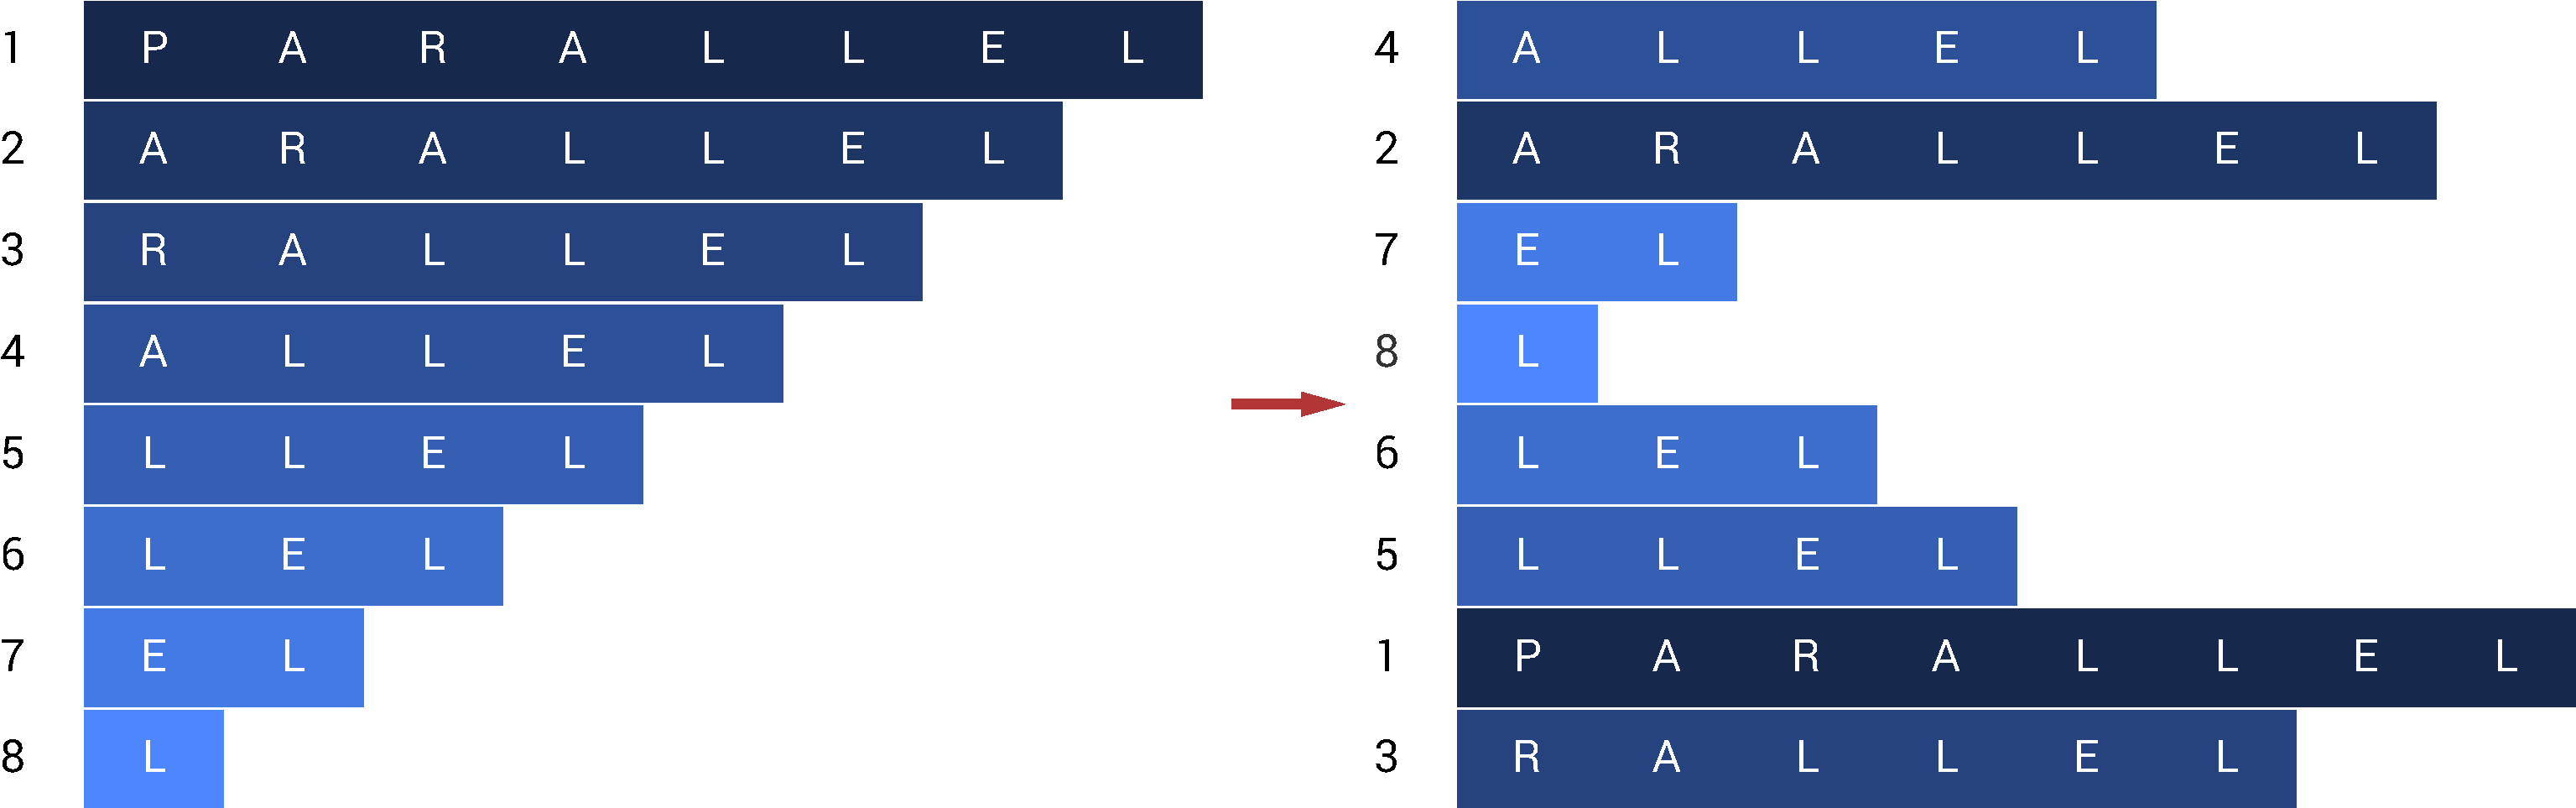
\includegraphics[width=\linewidth,bb=0 0 1474 462]{./assets/whatIsASuffixArray.pdf}
	\caption{Suffixarray für $S =$ `parallel'}
\label{fig:whatIsASuffixArray}
\end{figure}

Um Speicher zu sparen wird $SA$ allerdings nicht als Folge der Suffix-Zeichenketten, sondern als Folge der Startpunkte der Suffixe repräsentiert. Für $S =$ `parallel' wäre also $SA = (4, 2, 7, 8, 6, 5, 1, 3)$. Formal bedeutet dies:
\begin{align*}
	\Sigma &:= \text{streng total geordnetes endliches Alphabet} \\
	S &:= \text{Eingabezeichenkette} = (S[1], \dots, S[n]) \in \Sigma^n, |S| := n \in \mathbb{N} \\
	S[i .. j + 1) := S[i .. j] &:= (S[i], \dots, S[j]) \\
	S_i &:= \text{$i$-ter Suffix von $S$} = S[i .. n] \\
	S \sqsubseteq T &:\Leftrightarrow \text{$S$ ist Präfix von $T$} \Leftrightarrow S = T[1 .. |S|] \\
	S <_{lex} T &:\Leftrightarrow (\exists\ i: S[i] < T[i] \land S[1 .. i) = T[1 .. i)) \lor (|S| < |T| \land S \sqsubseteq T) \\
	SA &:= \text{Permutation von } \{1, \dots, |S|\} \text{, sodass } \forall\ i < j: S_{SA[i]} <_{lex} S_{SA[j]}
\end{align*}

\subsection{Einsatzgebiete von Suffixarrays}

Suffixarrays finden in vielen Bereichen als Index-Datenstruktur Verwendung~\cite{wikiSuffixArray}. Ein typisches Problem, dessen Lösung durch Suffixarrays beschleunigt werden kann, ist z.~B. die Substringsuche. Bei dieser soll bestimmt werden, \textit{ob} und wenn ja, \textit{wo} in einem Text $T$ ein Pattern $P$ vorkommt. Ohne einen Index benötigt dieses Problem z.~B. mit Knuth-Morris-Pratt $\mathcal{O}(|T| + |P|)$. Mit einem Suffixarray als Index über $T$ hingegen lassen sich Matches durch eine binäre Suche in $\mathcal{O}(|P| \log |T|)$ finden. Da i.~d.~R. $|P| \ll |T|$, ist dies ein deutlicher Speedup, welcher z.~B. in Datenbanksystemen für Volltextsuchen und in der Bioinformatik für das Suchen in DNA-Daten nützlich ist.

\begin{figure}[h]
	\centering
	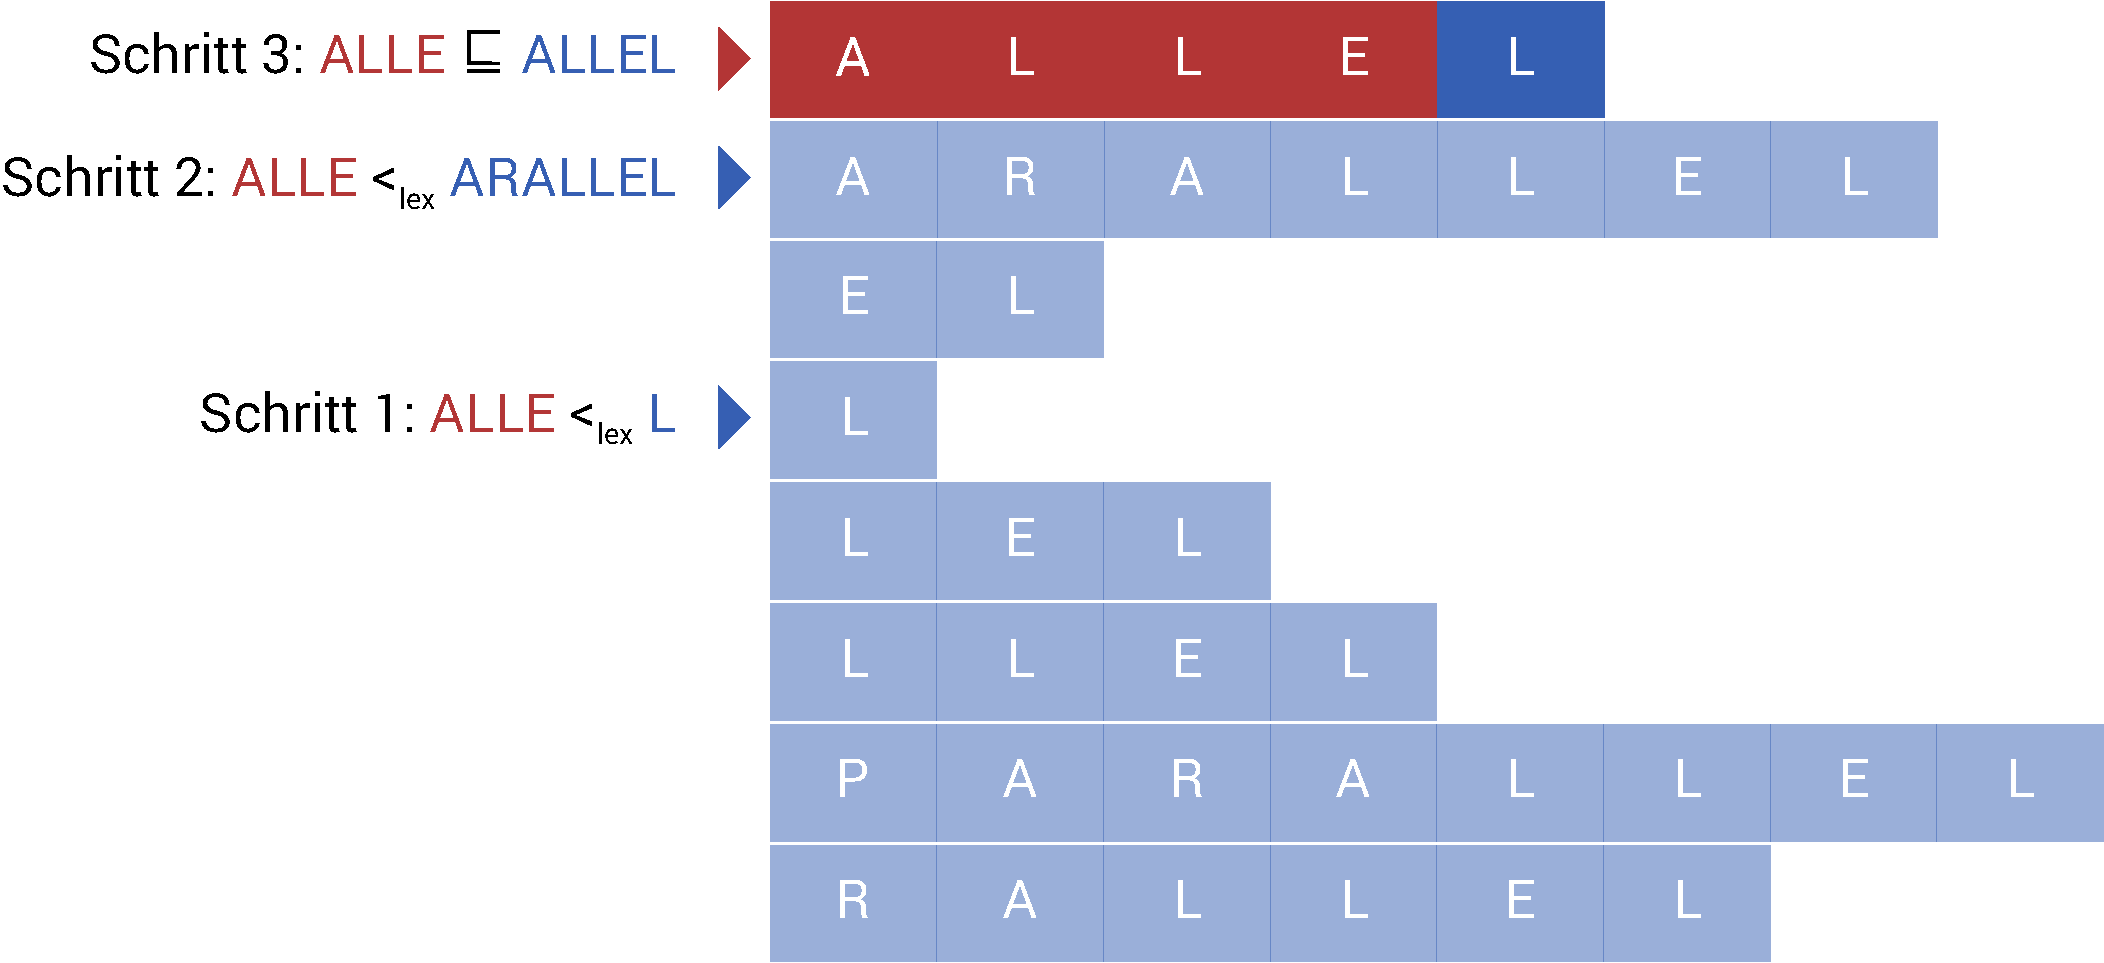
\includegraphics[width=0.7\linewidth,bb=0 0 1010 462]{./assets/substringSearch.pdf}
	\caption{Substringsuche mit $P =$ `alle' und $T =$ `parallel'}
\label{fig:substringSearch}
\end{figure}

Ein weiteres Einsatzgebiet für Suffixarrays ist als Suchstruktur für das Sliding Window in Implementationen des LZ77-Kompressionsalgorithmus.

\section{Ansätze zur Suffixarray-Konstruktion}

Nachdem nun der Begriff des Suffixarrays definiert wurde, wird im Folgenden betrachtet wie sich dieses prinzipiell algorithmisch berechnen lässt.

\subsection{Naiver Ansatz}

Da es sich bei der Suffixarray-Berechnung im Wesentlichen um ein Sortierproblem handelt, liegt die Idee nahe dies mit einem allgemeinen Sortierverfahren zu lösen. Dazu bietet sich z.~B. der Quicksort-Algorithmus an. Im average case wären dann $\mathcal{O}(n \log n)$ Vergleiche notwendig. Für den lexiographischen Vergleich zweier Suffixe müssen wiederum bis zu $\mathcal{O}(n)$ Zeichen miteinander verglichen werden. Insgesamt ergibt sich also eine Laufzeit von $\mathcal{O}(n^2 \log n)$. Dies ist weit von der angestrebten $\mathcal{O}(n)$-Laufzeit entfernt. Allgemeine Sortierverfahren sind daher für die Suffixarray-Konstruktion unbrauchbar.

\subsection{Überblick über bisherige Linearzeitansätze}

Es sind bereits zahlreiche Linearzeitalgorithmen zur Konstruktion von Suffixarrays bekannt. Allerdings sind all diese Verfahren rekursiv. Das bedeutet, dass sie neben der Eingabe und evtl. Hilfsdatenstrukturen zudem mindestens $\mathcal{O}(\log n)$ Speicher für die Stackframes der rekursiven Aufrufe benötigen.\\

Zwei dieser rekursiven Linearzeitalgorithmen sind der Algorithmus von Skew und der SAIS-Algorithmus. Skew ist primär wegen seiner Kompaktheit und Eleganz interessant. SAIS basiert auf dem Konzept der induzierten Sortierung und gehört zu den schnellsten bekannten SACAs (suffix array construction algorithms). Obwohl es sich bei beiden um Linearzeitalgorithmen handelt, sind die konstanten Faktoren in Implementationen von SAIS deutlich geringer.

\begin{table}[h]
\begin{center}
\begin{tabular}{r | c c c}
& Skew & SAIS & \textbf{GSACA} \\
\hline
Art & \textcolor{rot}{rekursiv} & \textcolor{rot}{rekursiv} & \textcolor{gruen}{iterativ} \\
Zeit & $\mathcal{O}(n)$ & $\mathcal{O}(n)$ & $\mathcal{O}(n)$ \\
Speicher & $\textcolor{rot}{\mathcal{O}(\log n)} + \max 24n$ & $\textcolor{rot}{\mathcal{O}(\log n)} + \max 2n$ & $\textcolor{gruen}{\mathcal{O}(1)}\ +\ ?$
\end{tabular}

\caption{Vergleich von Skew, SAIS und GSACA}
\label{tab:skewSaisGsacaComparison}
\end{center}
\end{table}

\section{Der GSACA-Algorithmus}

Im Rest dieser Arbeit wird es um den GSACA-Algorithmus (greedy suffix array construction algorithm) gehen, welcher der erste bekannte rekursionsfreie Linearzeit-SACA ist. Skew und SAIS werden dabei als Referenzalgorithmen dienen, mit denen GSACA verglichen wird.

\subsection{Grundlegende Konzepte}

Um den GSACA-Algorithmus zu verstehen, ist es hilfreich zuerst eine Intuition dafür zu geben, wieso Suffixe überhaupt in $\mathcal{O}(n)$ sortiert werden können. Im Gegensatz zu allgemeinen Sortierverfahren mit $\mathcal{O}(n \log n)$ Vergleichen, lassen sich hier offenbar Vergleiche sparen.

\subsubsection{Induziertes Sortieren}

Der fundamentale Unterschied zwischen allgemeinen Sortierproblemen und der Suffixsortierung ist, dass aus der Ordnung von bestimmten Suffixen $T(1) <_{lex} \dots <_{lex} T(n)$ die Ordnung anderer Suffixe $G(1), \dots, G(n)$ induziert werden kann. Es muss dann also lediglich Zeit in Vergleiche der $T$-Suffixe investiert werden.

\begin{align*}
	T :=\ &\{ T(1), \dots, T(n) \}, \text{sodass } T(1) <_{lex} \dots <_{lex} T(n) \\
	G :=\ &\{ G(1), \dots, G(n) \}, \text{sodass } \exists\ P \in \Sigma^*\ \forall\ i: G(i) = P\ T(i) \\
	\implies &G(1) <_{lex} \dots <_{lex} G(n)
\end{align*}

Um diese Implikation nutzen zu können, müssen Suffixe also mit einem geschickt gewählten Präfix $P$ einer Gruppe $G$ zugeordnet werden. GSACA tut genau das.

\subsubsection{Gruppenkontext}

Für die Gruppierung von Suffixen benutzt GSACA das Konzept des \textit{Gruppenkontextes}, welcher als der gemeinsame Präfix $P$ aller Suffixe in einer Gruppe dient. Dieser Begriff wird im Folgenden näher betrachtet. Es wird dabei angenommen, dass es sich bei der Eingabe $S$ um einen \textit{nullterminierten} String handelt.

\begin{align*}
	S \text{ nullterminiert} &:\Leftrightarrow S[n] = \$ \land S[1..n) \in (\Sigma \setminus \{\$\})^*, \text{mit } \$ \in \Sigma, \forall\ \sigma \in \Sigma \setminus \{\$\}: \$ < \sigma \\
	\text{zur Erinnerung: } S_i &:= \text{$i$-ter Suffix von $S$} = S[i .. n] \\
	\widehat{i} &:= \min \{ j \in \{ i, \dots, n \}:\ S_j <_{lex} S_i \} \\
	\text{Gruppenkontext von } S_i &:= S[i .. \widehat{i}) \\
	\text{Gruppe von } S_i &:= \{ S_j:\ \text{Gruppenkontext } S_i = \text{Gruppenkontext } S_j \}
\end{align*}

\begin{figure}[h]
	\centering
	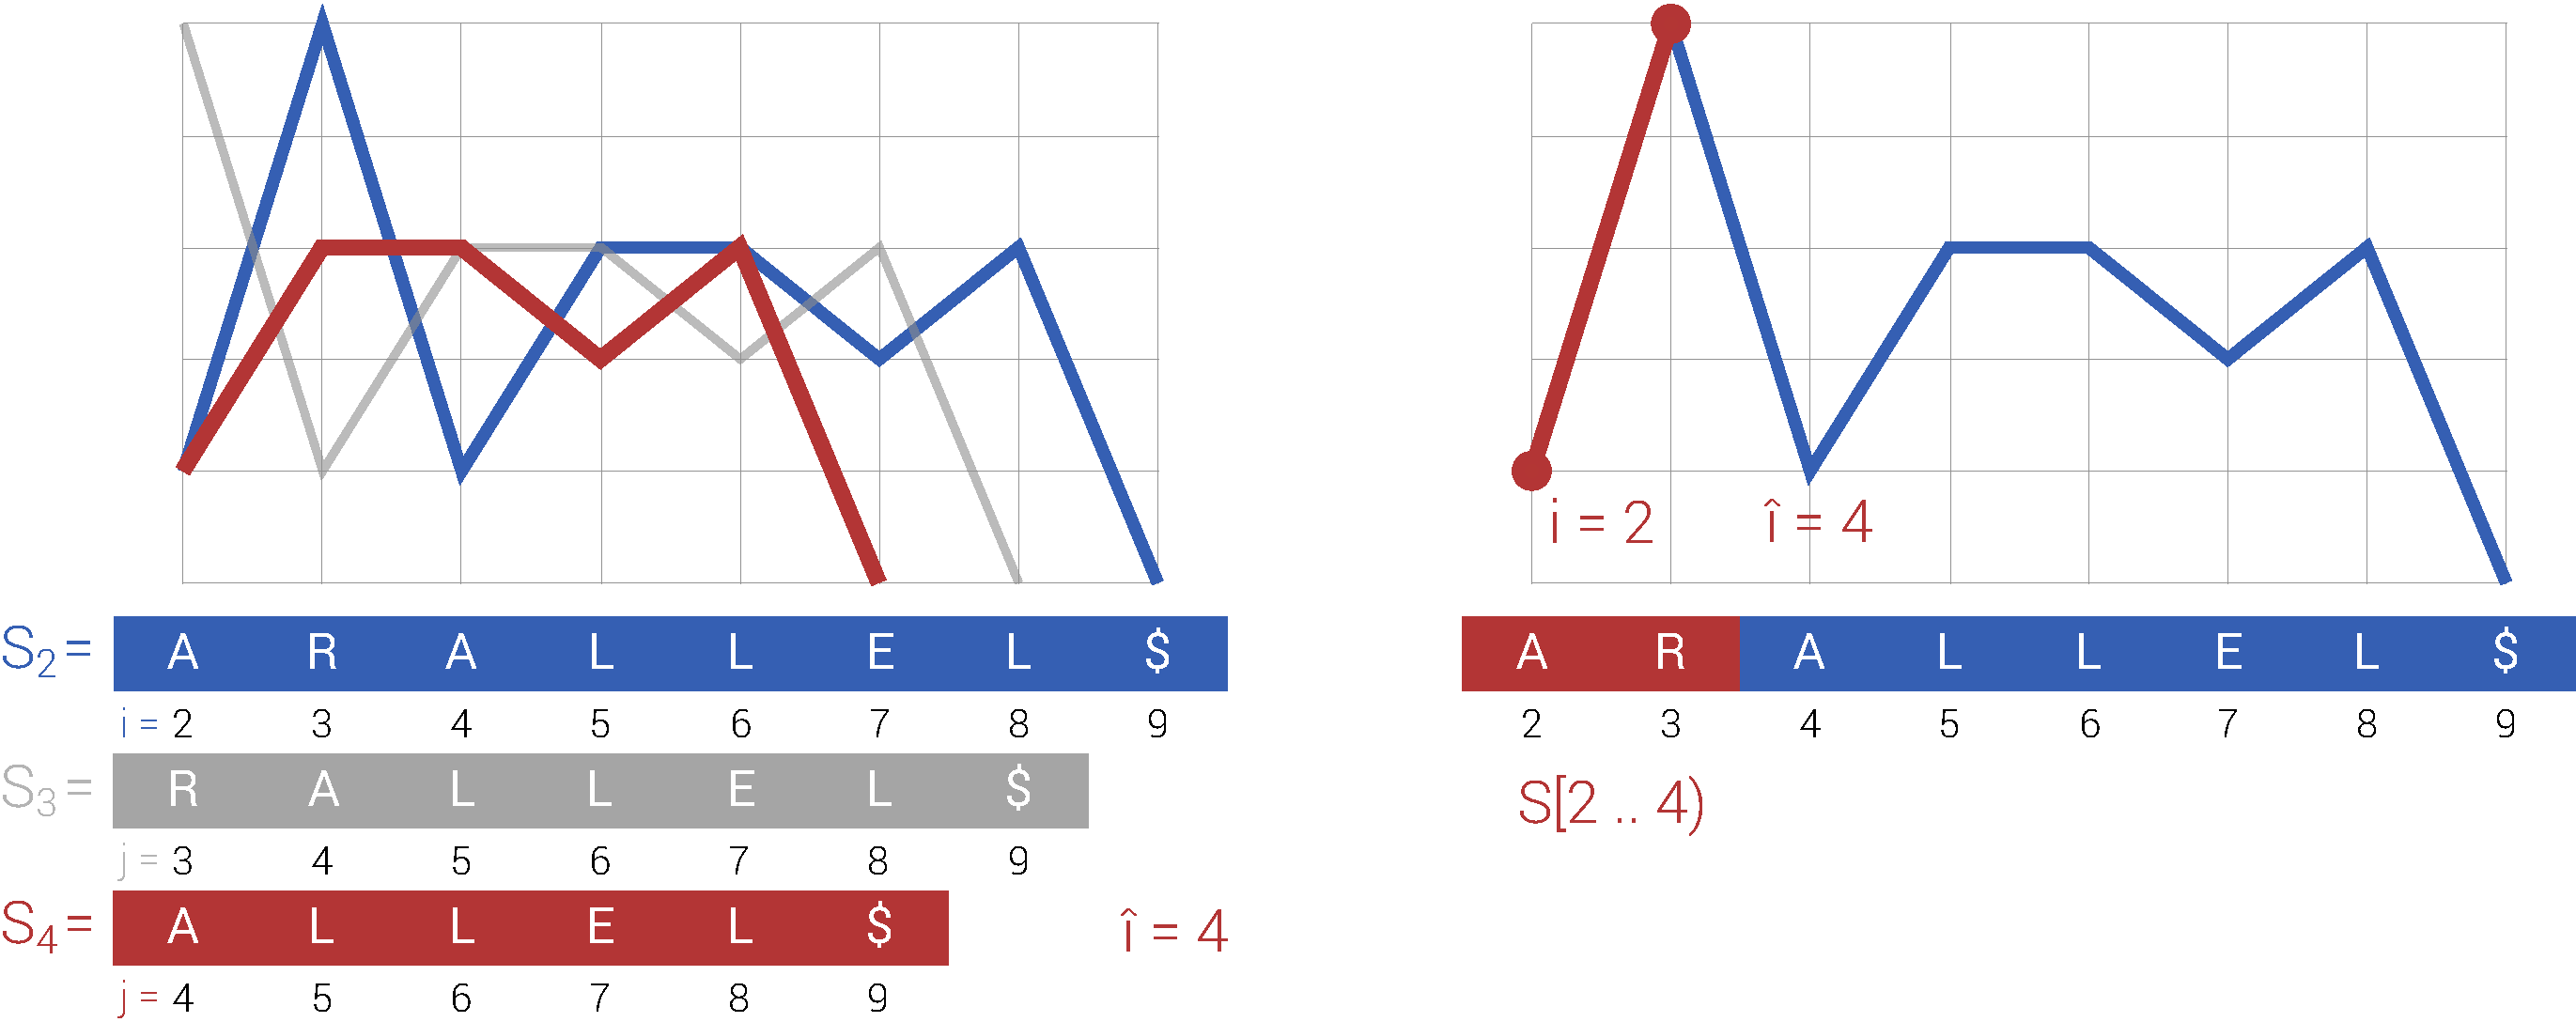
\includegraphics[width=\linewidth,bb=0 0 1316 522]{./assets/groupContext.pdf}
	\caption{Veranschaulichung des Gruppenkontextes von $S_2$ für $S =$ `parallel\$'}
\label{fig:groupContext}
\end{figure}

Der Gruppenkontext eines Suffixes $S_i$ ist also dessen erster Präfix auf den ein lexiographisch kleinerer Suffix von $S_i$ folgt.

\subsection{Die zwei Phasen von GSACA}

Mit dem Konzept des induzierten Sortierens und dem des Gruppenkontextes zur Gruppierung von Suffixen, lässt sich GSACA nun als ein in zwei Phasen ablaufender Algorithmus verstehen. \\

In der \textit{ersten Phase} werden alle Suffixe der Eingabe gemäß ihrer Gruppenkontexte in Gruppen zusammengefasst. Die resultierenden Gruppen werden dabei nach Gruppenkontext aufsteigend sortiert zurückgegeben. \\

Diese sortierte Folge von Gruppen wird nun als Eingabe der \textit{zweiten Phase} verwendet. Da die Gruppen untereinander bereits nach ihrem Kontext sortiert wurden und ein Kontext jeweils Präfix der Suffixe seiner Gruppe ist, müssen die Suffixe in dieser Phase lediglich innerhalb ihrer jeweiligen Gruppe geordnet werden. Für das Ordnen der Suffixe innerhalb einer Gruppe wird induziertes Sortieren genutzt.

\begin{figure}[h]
	\centering
	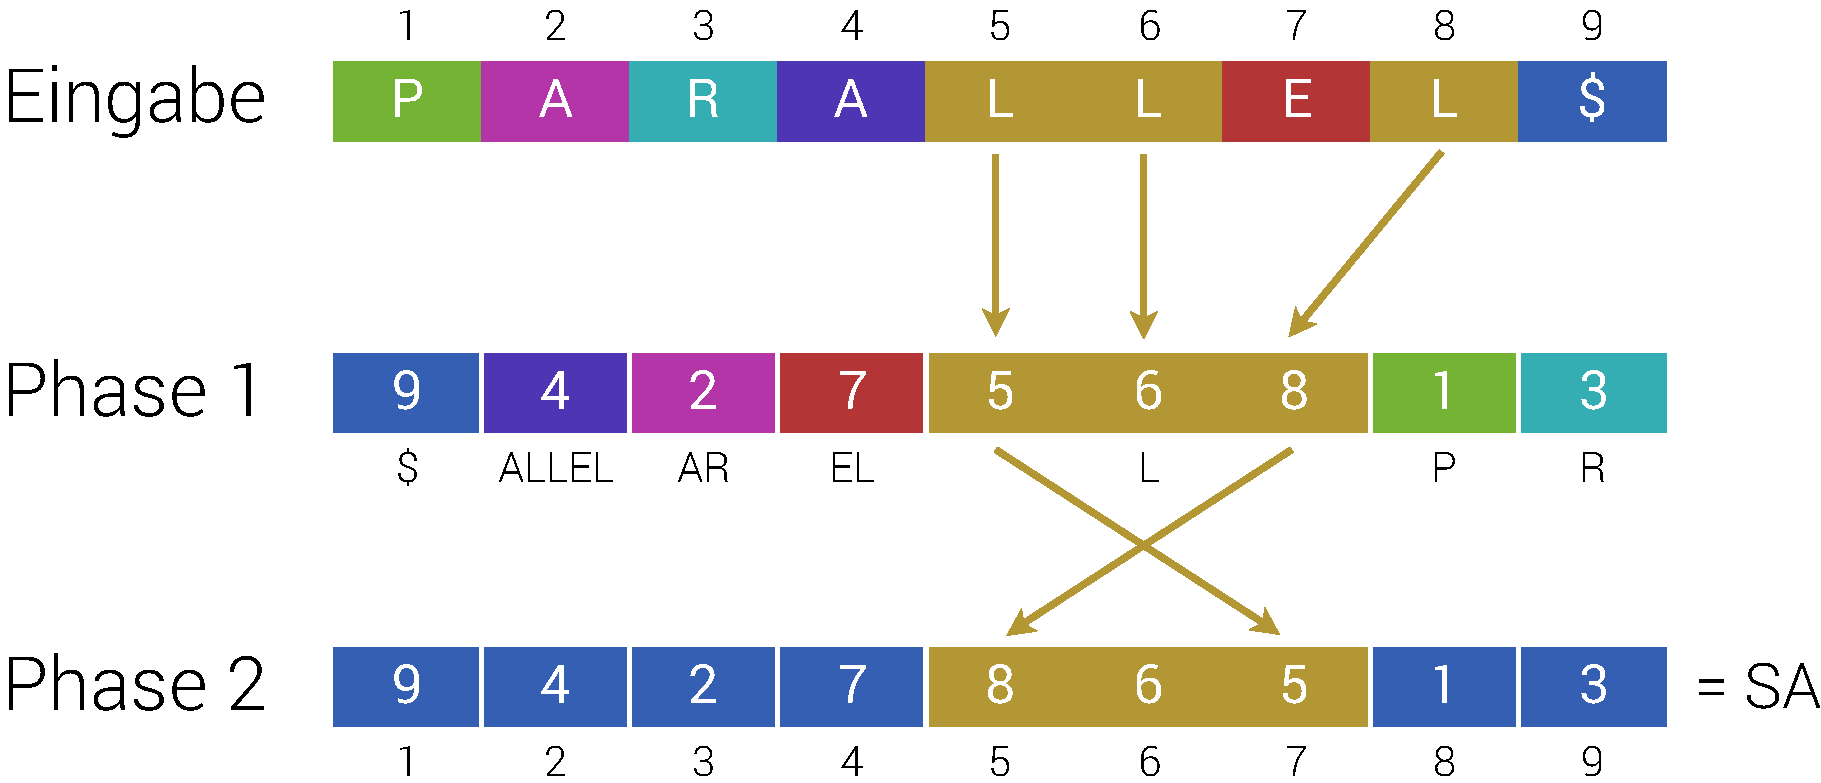
\includegraphics[width=0.7\linewidth,bb=0 0 874 376]{./assets/twoPhases.pdf}
	\caption{Ausgabe beider Phasen für $S =$ `parallel\$', Farben kennzeichnen Gruppen}
\label{fig:twoPhases}
\end{figure}

Das Ergebnis der zweiten Phase ist das gesuchte Suffixarray. Ziel ist es nun beide Phasen ohne Rekursion als $\mathcal{O}(n)$-Algorithmen zu formulieren.

\subsubsection{Phase 1}

\paragraph{Intuition} GSACA berechnet die Gruppen, indem jedem Suffix zu Anfang ein vorläufiger einstelliger Gruppenkontext zugewiesen wird. Diese vorläufigen Kontexte werden dann sukzessive erweitert, bis am Ende jeder Suffix den korrekten Gruppenkontext hat.\\

Konkret bedeutet dies, dass der Kontext jedes Suffixes $S_i$ zu Beginn auf $S[i]$ gesetzt wird. Da das Eingabealphabet $\Sigma$ als konstant angenommen wird, können die Suffixe nun z. B. mit einem Bucketsort in $\mathcal{O}(n)$ gemäß ihres Kontextes in eine aufsteigende Folge von vorläufigen Gruppen sortiert werden.

\begin{figure}[h]
	\centering
	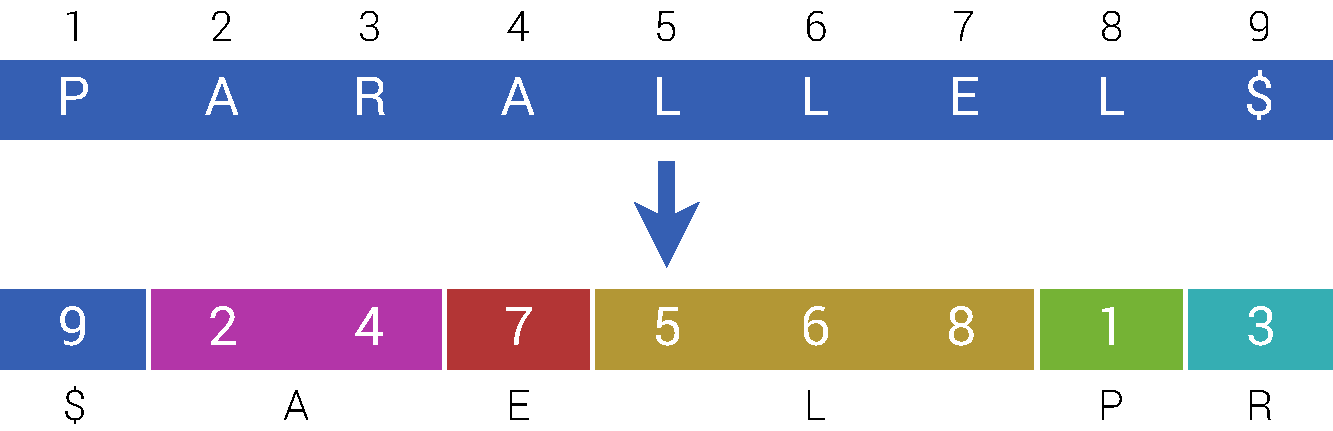
\includegraphics[width=0.5\linewidth,bb=0 0 640 207]{./assets/bucketsort.pdf}
	\caption{Ergebnis des Bucketsorts für $S =$ `parallel\$'}
\label{fig:bucketsort}
\end{figure}

Manche der sich ergebenden Gruppen müssen nun durch Kontexterweiterungen aufgespalten werden. Dies geschieht indem von hinten nach vorne, i.~e.\ von großem zu kleinem Kontext, über die Gruppen iteriert wird. Für jeden Suffix der aktuell iterierten Gruppe wird nun der sog. $prev$-Pointer berechnet.
$$prev(i) := \max \{ j \in \{ 1, \dots, i \}: \text{akt. Gruppenkontext } S_j <_{lex} \text{akt. Gruppenkontext } S_i \}$$
$prev(i)$ ist verwandt mit der $\widehat{i}$-Funktion. Statt des \textit{nächst kleineren} Suffix, gibt $prev$ allerdings den ersten \textit{vorherigen} Suffix aus einer Gruppe mit \textit{kleinerem aktuellen Kontext} zurück. Aus dieser Verwandtschaft folgt, dass $j = prev(i) < i < \widehat{i} \le \widehat{j}$ gilt. Das bedeutet, dass der Gruppenkontext von $S_i$ Teil des Gruppenkontextes von $S_{prev(i)}$ ist. Es lässt sich zeigen, dass durch das Iterieren von großen zu kleinen Gruppen in jeder Iteration für jeden Suffix $S_i$ der gerade iterierten Gruppe gilt:
$$concat(\text{aktueller Kontext } S_{prev(i)},\ \text{aktueller Kontext } S_i) \sqsubseteq \text{Gruppenkontext } S_{prev(i)}$$
Deshalb kann der aktuelle Kontext von $S_{prev(i)}$ um den aktuellen Kontext von $S_i$ erweitert werden. Der neue erweiterte Kontext von $S_{prev(i)}$ ist nun lexiographisch größer als vorher, $S_{prev(i)}$ wird deshalb aus seiner bisherigen Gruppe $G$ entfernt und in eine neue Gruppe $G'$ eingefügt, die in der Gruppenfolge hinter $G$ eingeordnet wird.

\begin{figure}[h]
	\centering
	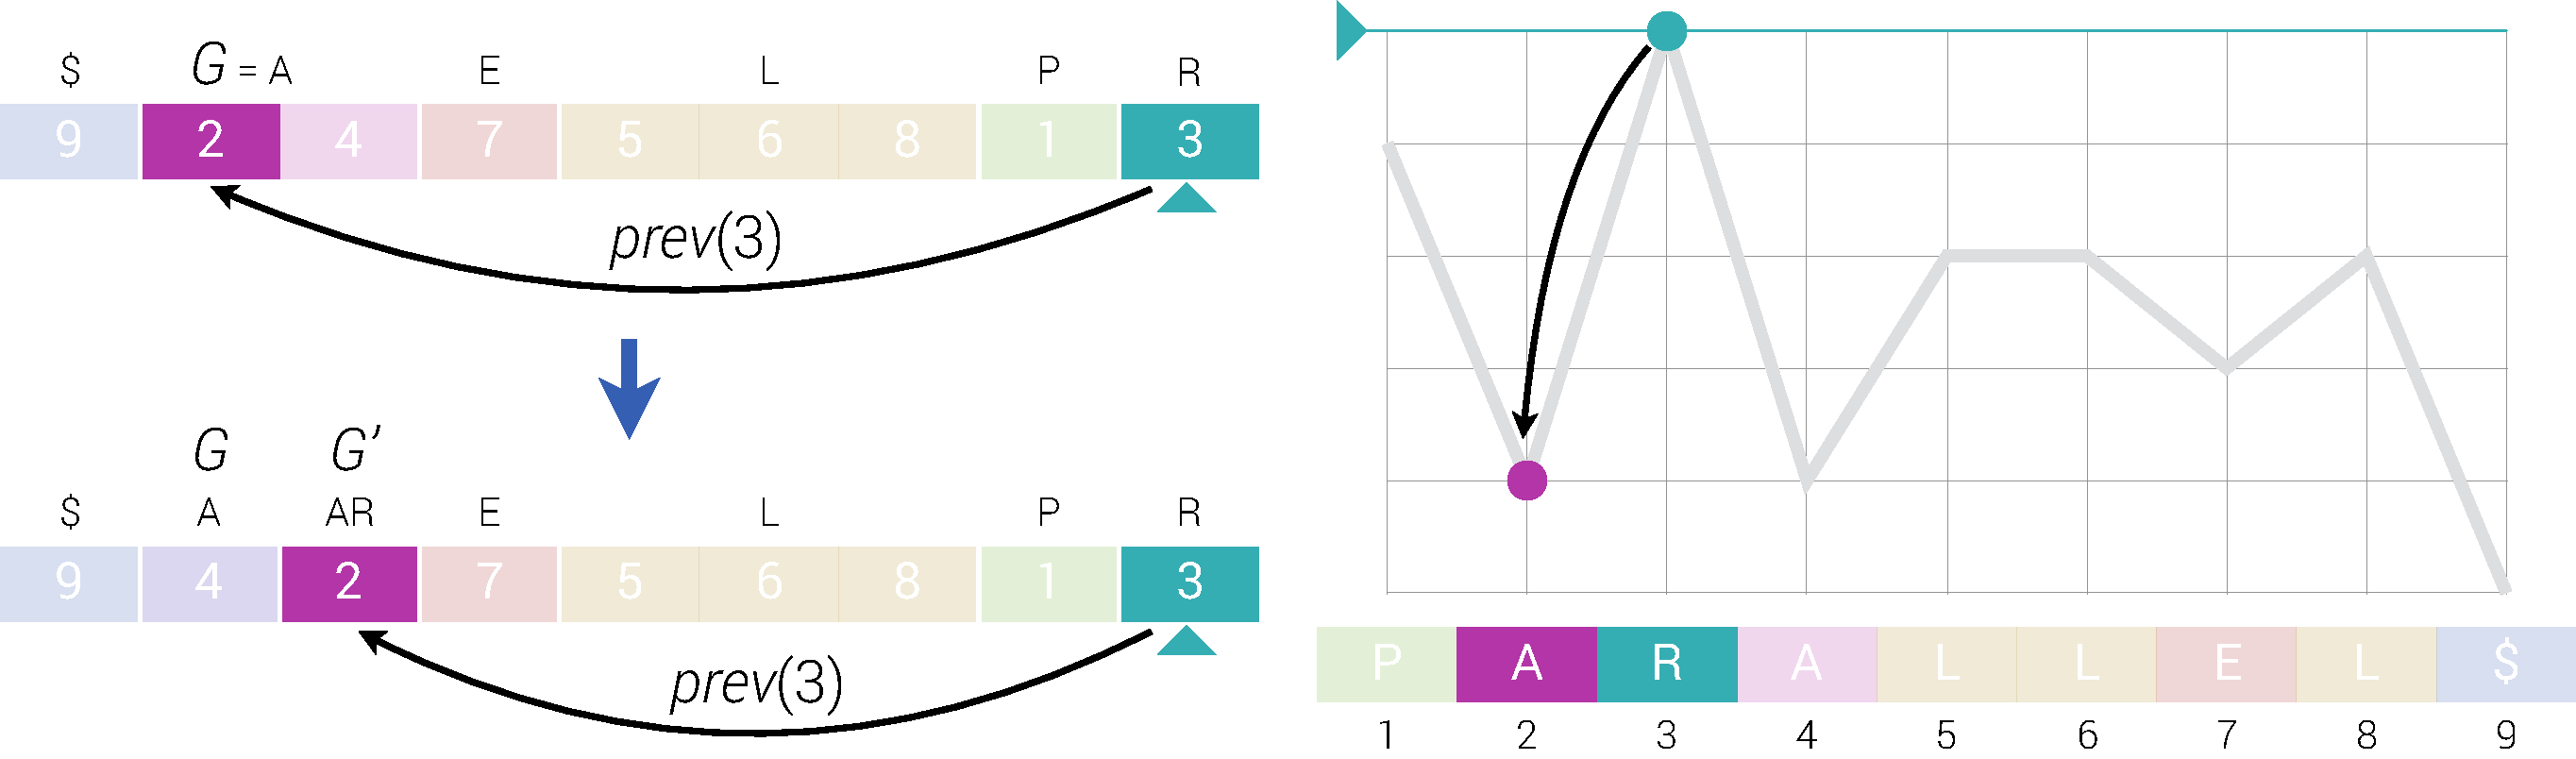
\includegraphics[width=\linewidth,bb=0 0 1310 386]{./assets/phase1-R.pdf}
	\caption{Iteration 1 von Phase 1: Kontexterweiterung mit Suffixen der \textit{R}-Gruppe}
\label{fig:phase1-R}
\end{figure}

Bei der soeben beschriebenen Kontexterweiterung kann nun folgender Fall eintreten: $k > 1$ der Suffixe der gerade iterierten Gruppe $G$ haben den selben $prev$-Pointer-Wert $p$. In dieser Situation wird der Kontext von $p$ $k$-mal um den $G$-Kontext erweitert. Durch einen Widerspruchsbeweis lässt sich nämlich leicht zeigen, dass der $G$-Kontext dann $k$-mal direkt hintereinander auf den $p$-Kontext folgt. Der Beweis wird hier ausgelassen.

\begin{figure}[h]
	\centering
	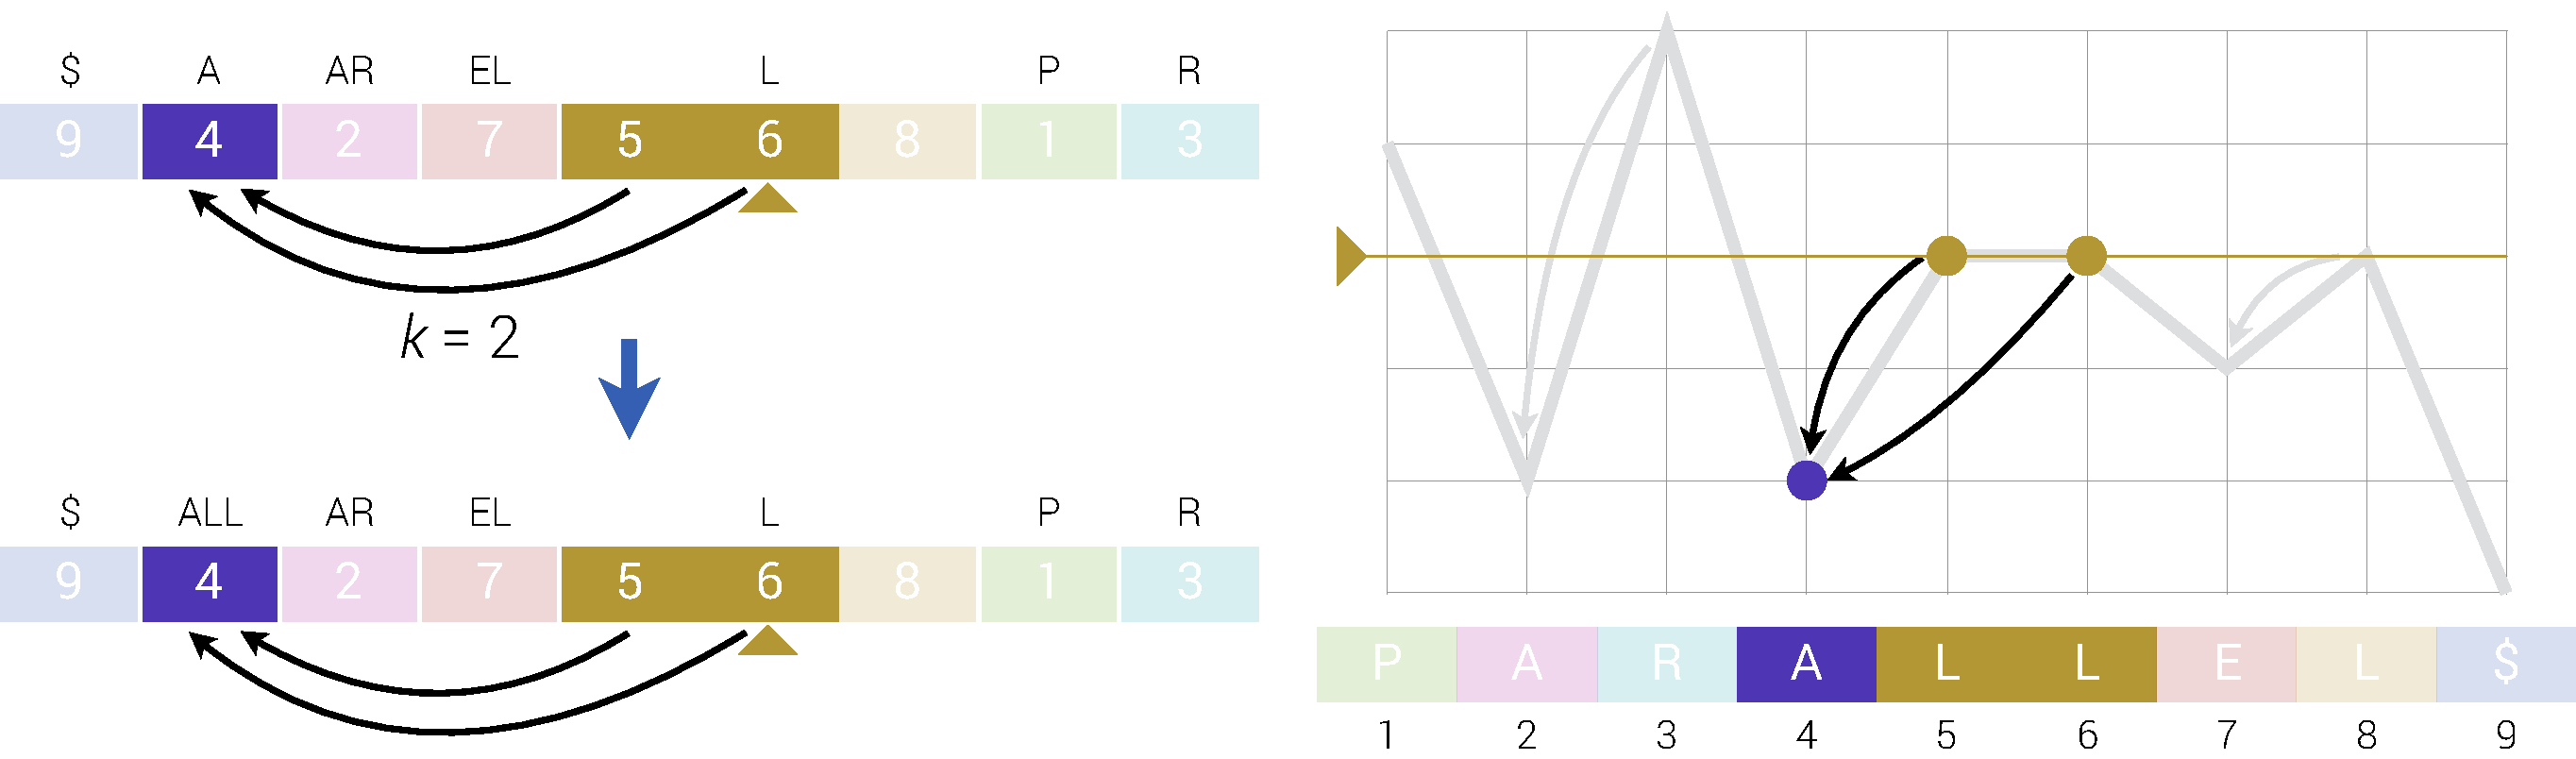
\includegraphics[width=\linewidth,bb=0 0 1310 386]{./assets/phase1-L.pdf}
	\caption{Iteration 3 von Phase 1: Doppelte Kontexterweiterung mit Suffixen der \textit{L}-Gruppe}
\label{fig:phase1-L}
\end{figure}

Nachdem so über alle Gruppen iteriert wurde, sind die aktuellen Kontexte aller Gruppen gleich den finalen Gruppenkontexten. Insgesamt kann jeder Suffix höchstens einmal zur Kontexterweiterung eines anderen Suffixes benutzt werden und jede Kontexterweiterung benötigt konstante Zeit. Für diesen Teil von Phase 1 ergibt sich also eine Laufzeit von $\mathcal{O}(n)$. Dabei wurde die $prev$-Pointer-Berechnung allerdings noch nicht berücksichtigt. Ein naiver Ansatz zum Berechnen von $prev(i)$ ist, rückwärts von $i - 1$ bis $1$ zu iterieren und beim ersten Suffix aus einer kleineren aktuellen Gruppe als der von $S_i$ zu stoppen. Mit dieser Strategie benötigt die $prev$-Berechnung $\mathcal{O}(n)$ Schritte. Da $n$ Pointer zu berechnen sind, würde Phase 1 so also $\mathcal{O}(n^2)$ Schritte brauchen.\\

Eine Optimierung ist notwendig: \textit{Pointer-Jumping}. Statt über alle $i - 1$ vorherige Suffixe zu iterieren, werden Suffixe übersprungen, die gar nicht als $prev$-Pointer in Frage kommen. Konkret wird beim Pointer-Jumping nicht über $i - 1,\, i - 2,\, i - 3, \dots$ sondern über $i - 1,\, prev(i - 1),\, prev^2(i - 1), \dots$ iteriert, wobei $prev^1(i) := prev(i),\ prev^k(i) := prev^{k - 1}(prev(i))$.\\

Es wird also der Kette der $prev$-Pointer ab Suffix $S_{i - 1}$ gefolgt, bis darin ein kleinerer Suffix gefunden wurde. Dies funktioniert, da alle Suffixe zwischen $prev^{k + 1}(i - 1)$ und $prev^k(i - 1)$ per Definition von $prev$ größer sein müssen als $prev^k(i - 1)$ und somit unmöglich als Wert von $prev(i)$ in Frage kommen, weil ja schon $prev^k(i - 1)$ zu groß ist.

\begin{figure}[h]
	\centering
	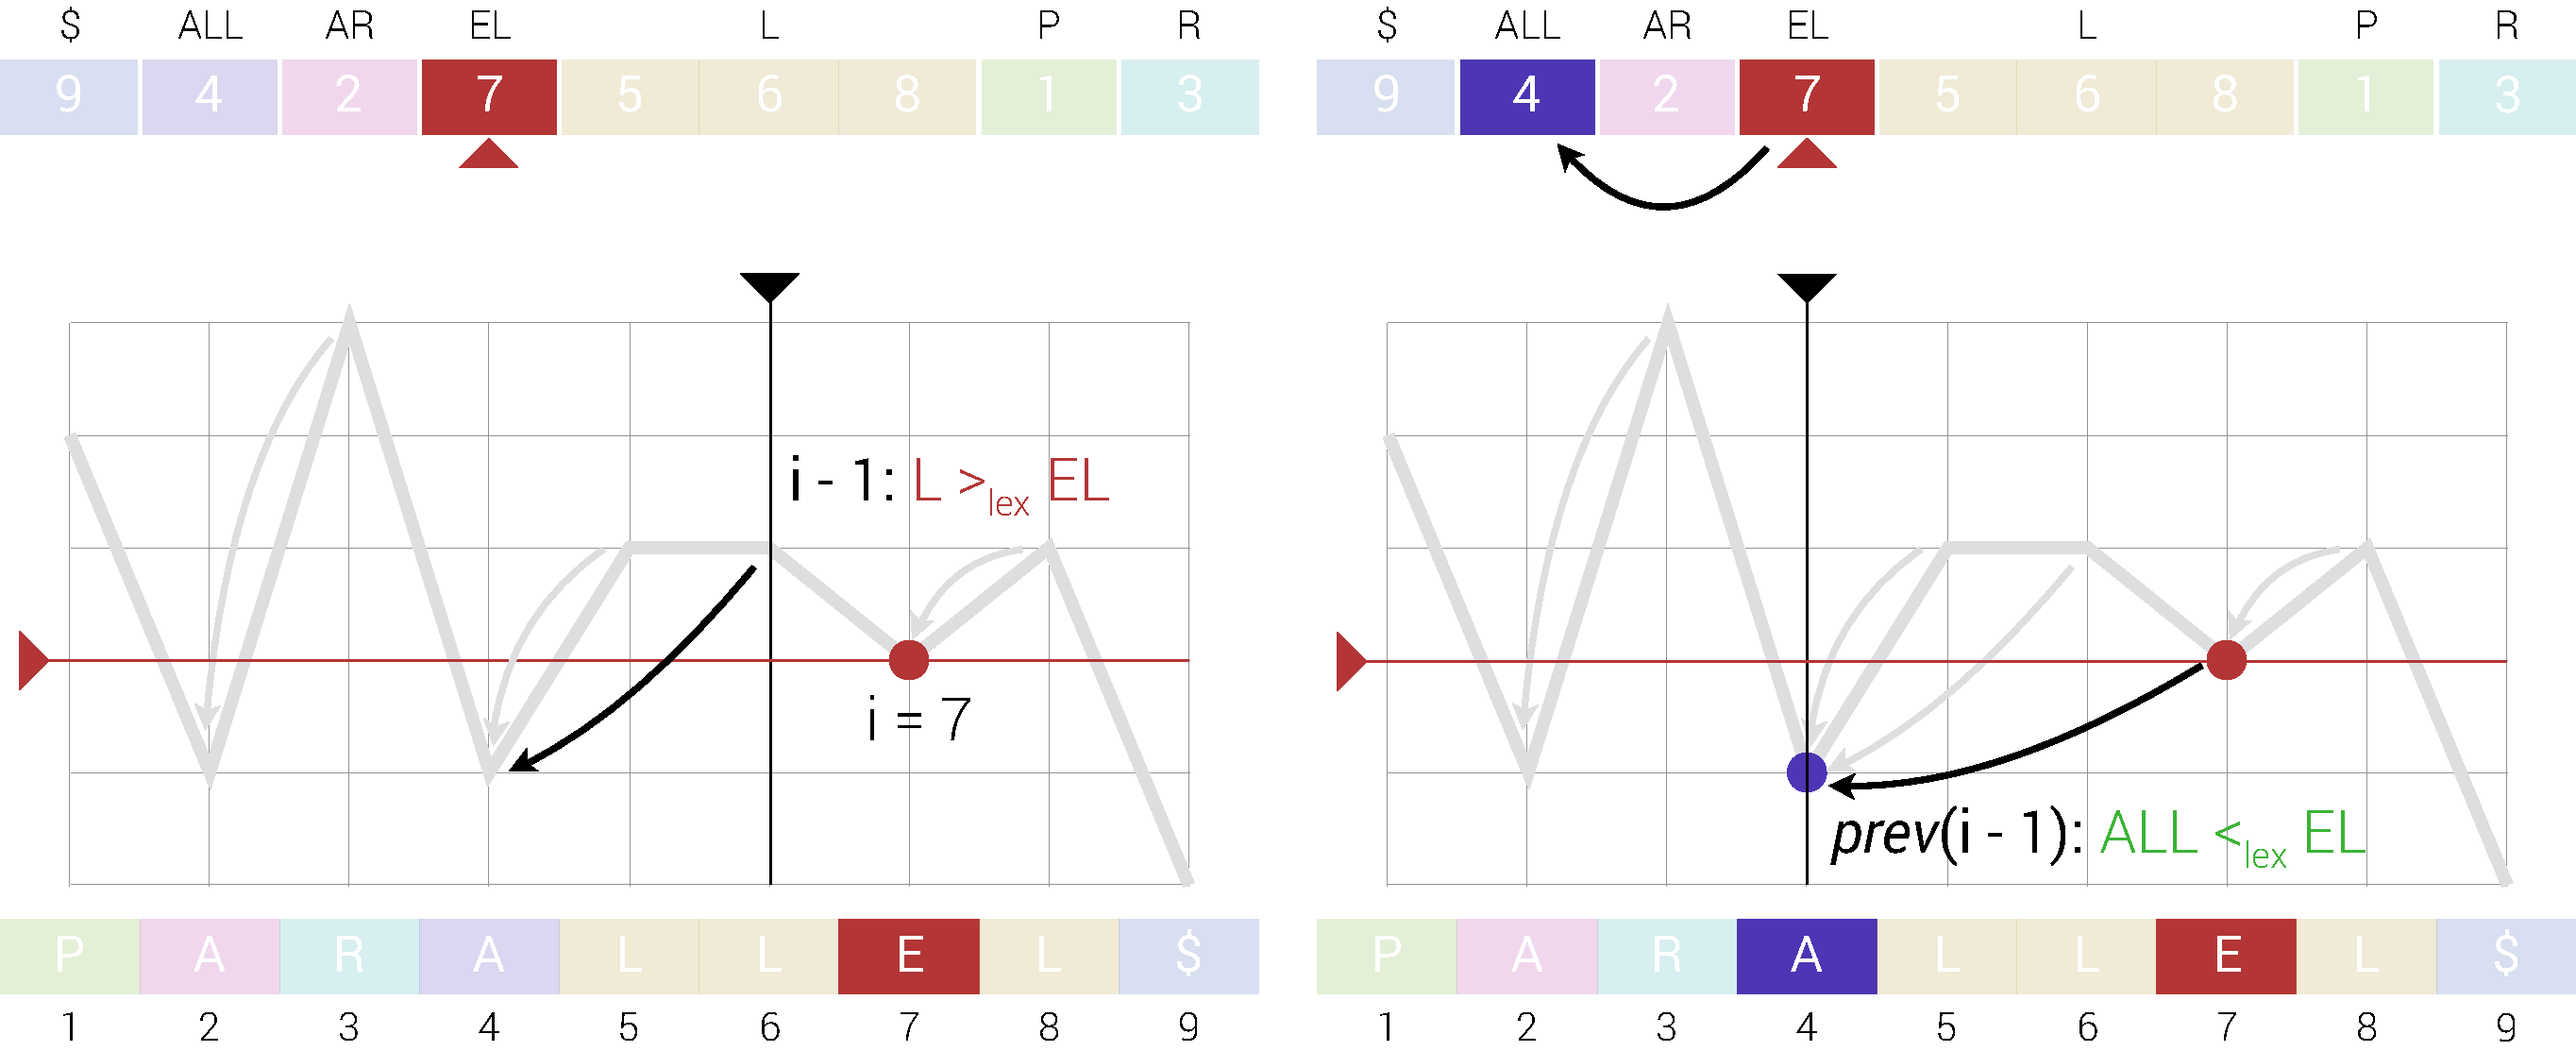
\includegraphics[width=\linewidth,bb=0 0 1310 534]{./assets/phase1-EL.pdf}
	\caption{Iteration 4 von Phase 1: $prev$-Pointer-Berechnung in der \textit{EL}-Gruppe}
\label{fig:phase1-EL}
\end{figure}

Durch das Pointer-Jumping können die $prev$-Pointer-Gesamtkosten in allen Gruppeniteration von Phase 1 von $\mathcal{O}(n^2)$ auf $\mathcal{O}(n)$ reduziert werden. Dies liegt daran, dass jeder $prev$-Pointer nur höchstens einmal für einen Pointer-Jump benutzt wird. Insgesamt können also höchstens $n$ Pointer-Jumps stattfinden. Der Beweis wird hier ausgelassen.
\begin{figure}[h]
	\centering
	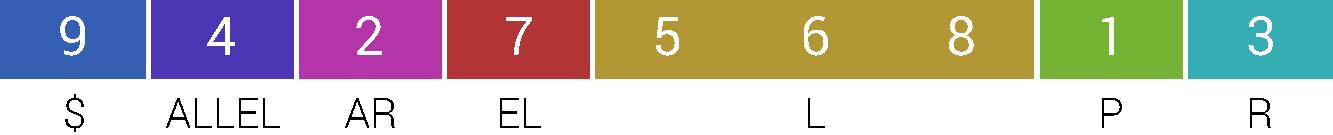
\includegraphics[width=0.5\linewidth,bb=0 0 640 67]{./assets/phase1Result.pdf}
	\caption{Ergebnis von Phase 1: Alle Suffixe sind gemäß ihrer Kontexte gruppiert und sortiert}
\label{fig:phase1Result}
\end{figure}

\subsubsection{Phase 2}

\paragraph{Intuition} In Phase 2 müssen die Suffixe nun innerhalb ihrer Gruppen geordnet werden. Hierzu wird zuerst das erste Element des gesuchten Suffixarrays bestimmt. Da die Gruppenkontexte geschickt definiert wurden, ermöglicht dies das Induzieren des zweiten Elements des Suffixarrays, woraus wiederum die Position des dritten Elements folgt, usw. \\

Konkret iteriert Phase 2, wie schon Phase 1, über alle Suffixe. Diesmal allerdings nicht von hinten nach vorne, sondern von vorne nach hinten, von den Suffixen der lexiographisch kleinsten Gruppe zu den Suffixen der größten Gruppe. \textit{Vor} jeder Iteration $i \in \{ 1, \dots, n \}$ gilt dabei die Invariante, dass die ersten $i$-Suffixe bereits an ihre finale Position im Suffixarray $SA$ einsortiert wurden. Für die erste Iteration $i = 1$ gilt dies, da GSACA per Definiton eine nullterminierte Eingabe erwartet und daher immer $SA[1] = \$$. \textit{Während} der $i$-ten Iteration wird zuerst die Suffixmenge $P_i$ berechnet.
\begin{align*}
	P_i :=\ & \{ \text{Suffix } S_j: \widehat{j} = SA[i] \} \\
	=\ & \{ \text{Suffix } S_j: S_j = concat(\text{Gruppenkontext von } S_j,\ S_{SA[i]}) \}
\end{align*}
Alle $S_j \in P_i$ werden danach aus ihrer Gruppe $G$ entfernt und vor $G$ eingefügt. Die resultierende Position $k$ von $S_j$ in der Gruppenliste ist die finale Position in $SA$, es kann also $SA[k] \leftarrow j$ gesetzt werden. Dies funktioniert, da die Suffixe von klein nach groß durchlaufen werden. Aus jeder Gruppe mit mehreren Suffixen wird daher zuerst der Suffix nach vorne gestellt, auf dessen Kontext der kleinste Suffix folgt und der somit per Definition von `$<_{lex}$' auch tatsächlich der kleinste Suffix seiner Gruppe ist. \\

Es gilt, dass $\widehat{SA[i + 1]} \in \{ SA[j]: j \in \{ 1, \dots, i \} \}$, da der Kontext des $(i + 1)$-ten Suffix nur von einem der kleineren Suffixe terminiert werden kann. Daher muss spätestens nach der $i$-ten Iteration $SA[i + 1]$ gefunden worden sein. Die zuvor definierte Invariante gilt also weiterhin. Nach der $(n - 1)$-ten Iteration müssen daher alle $n$ Suffixe korrekt einsortiert worden sein und $SA$ wurde berechnet.

\begin{figure}[h]
	\centering
	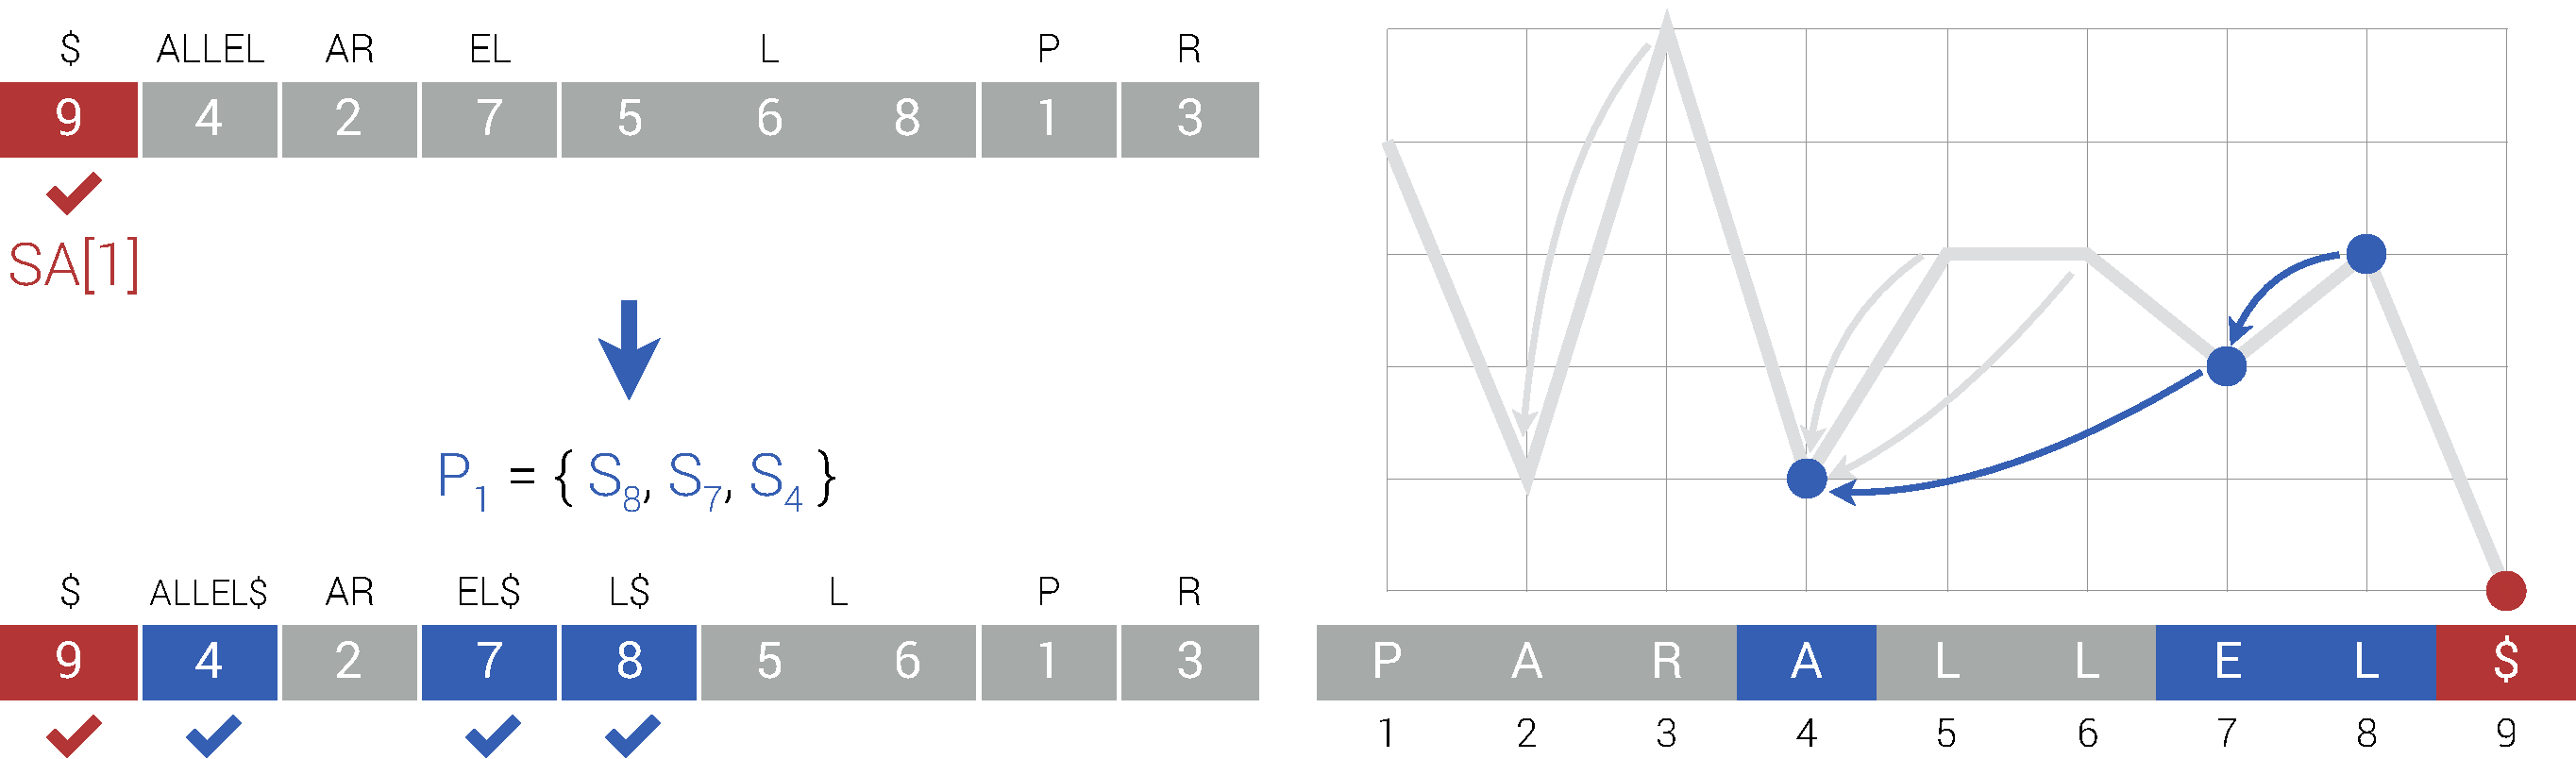
\includegraphics[width=\linewidth,bb=0 0 1310 386]{./assets/phase2-1.pdf}
	\caption{Iteration 1 von Phase 2: Einsortierung der $P_1$-Menge}
\label{fig:phase2-1}
\end{figure}

Die Laufzeit von Phase 2 hängt davon ab, wie schnell die $P_i$-Mengen ermittelt werden können. Die naive Strategie hierzu ist über alle Suffixe $S_j \ \in \{ S_1, \dots, S_{SA[i] - 1} \}$ zu iterieren und auf $\widehat{j} = SA[i]$ zu prüfen. Dafür sind $\mathcal{O}(n)$ notwendig. Da insgesamt $n - 1$ $P_i$-Mengen bestimmt werden müssen, ergibt sich mit der naiven Strategie also eine Laufzeit von $\mathcal{O}(n^2)$. \\
Wie schon bei der $prev$-Pointer-Berechnung in Phase 1 ist auch hier wieder eine Optimierung notwendig. Es lässt sich zeigen, dass die vorherige Definition von $P_i$ äquivalent ist zu:
\begin{align*}
	P_i &:= \pi(SA[i] - 1) \\
	\pi(j) &:= \begin{cases}
		\{ S_j \} \cup \pi(prev(j)): & S_j \text{ wurde noch nicht in $SA$ einsortiert} \land \exists\ prev(j) \\
		\{ S_j \}: & S_j \text{ wurde noch nicht in $SA$ einsortiert} \land \nexists\ prev(j) \\
		\emptyset: & \text{sonst}
	\end{cases}
\end{align*}
\begin{figure}[h]
	\centering
	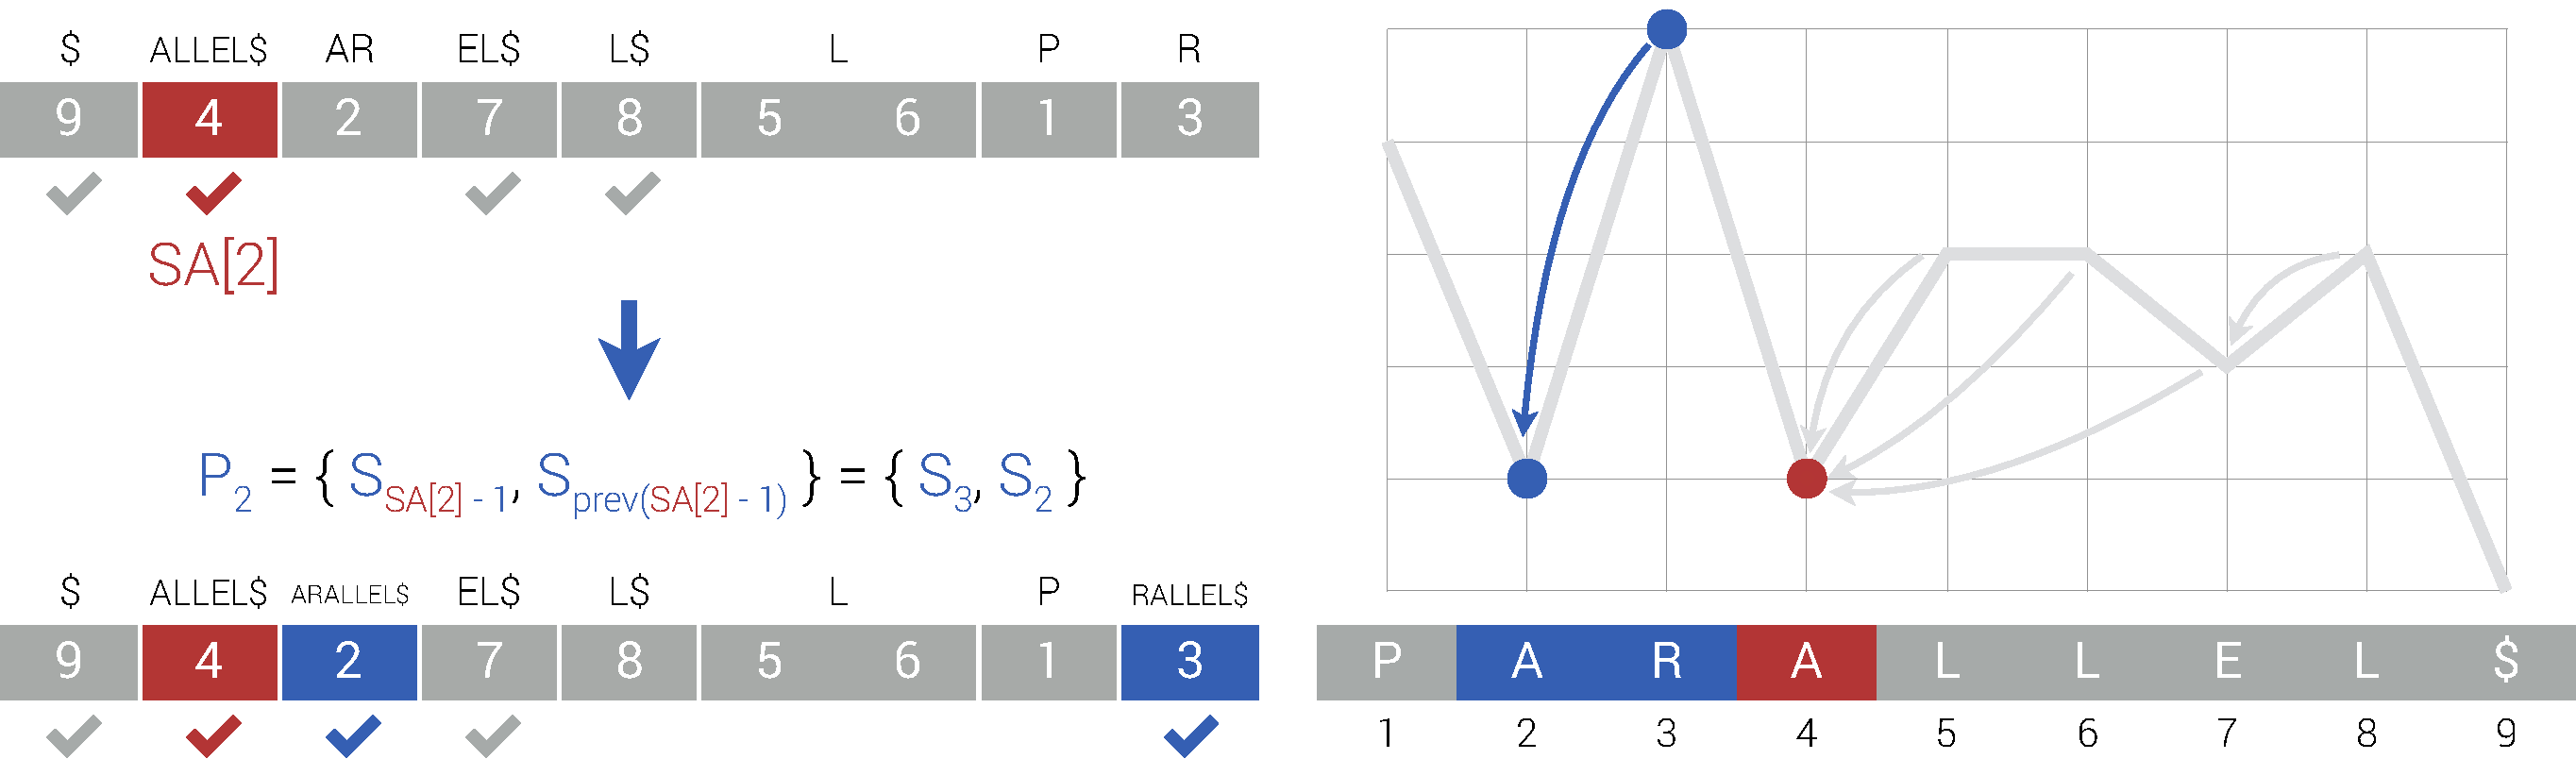
\includegraphics[width=\linewidth,bb=0 0 1310 386]{./assets/phase2-2.pdf}
	\caption{Iteration 2 von Phase 2: Berechnung und Einsortierung der $P_2$-Menge}
\label{fig:phase2-2}
\end{figure}
\hline
\begin{figure}[h]
	\centering
	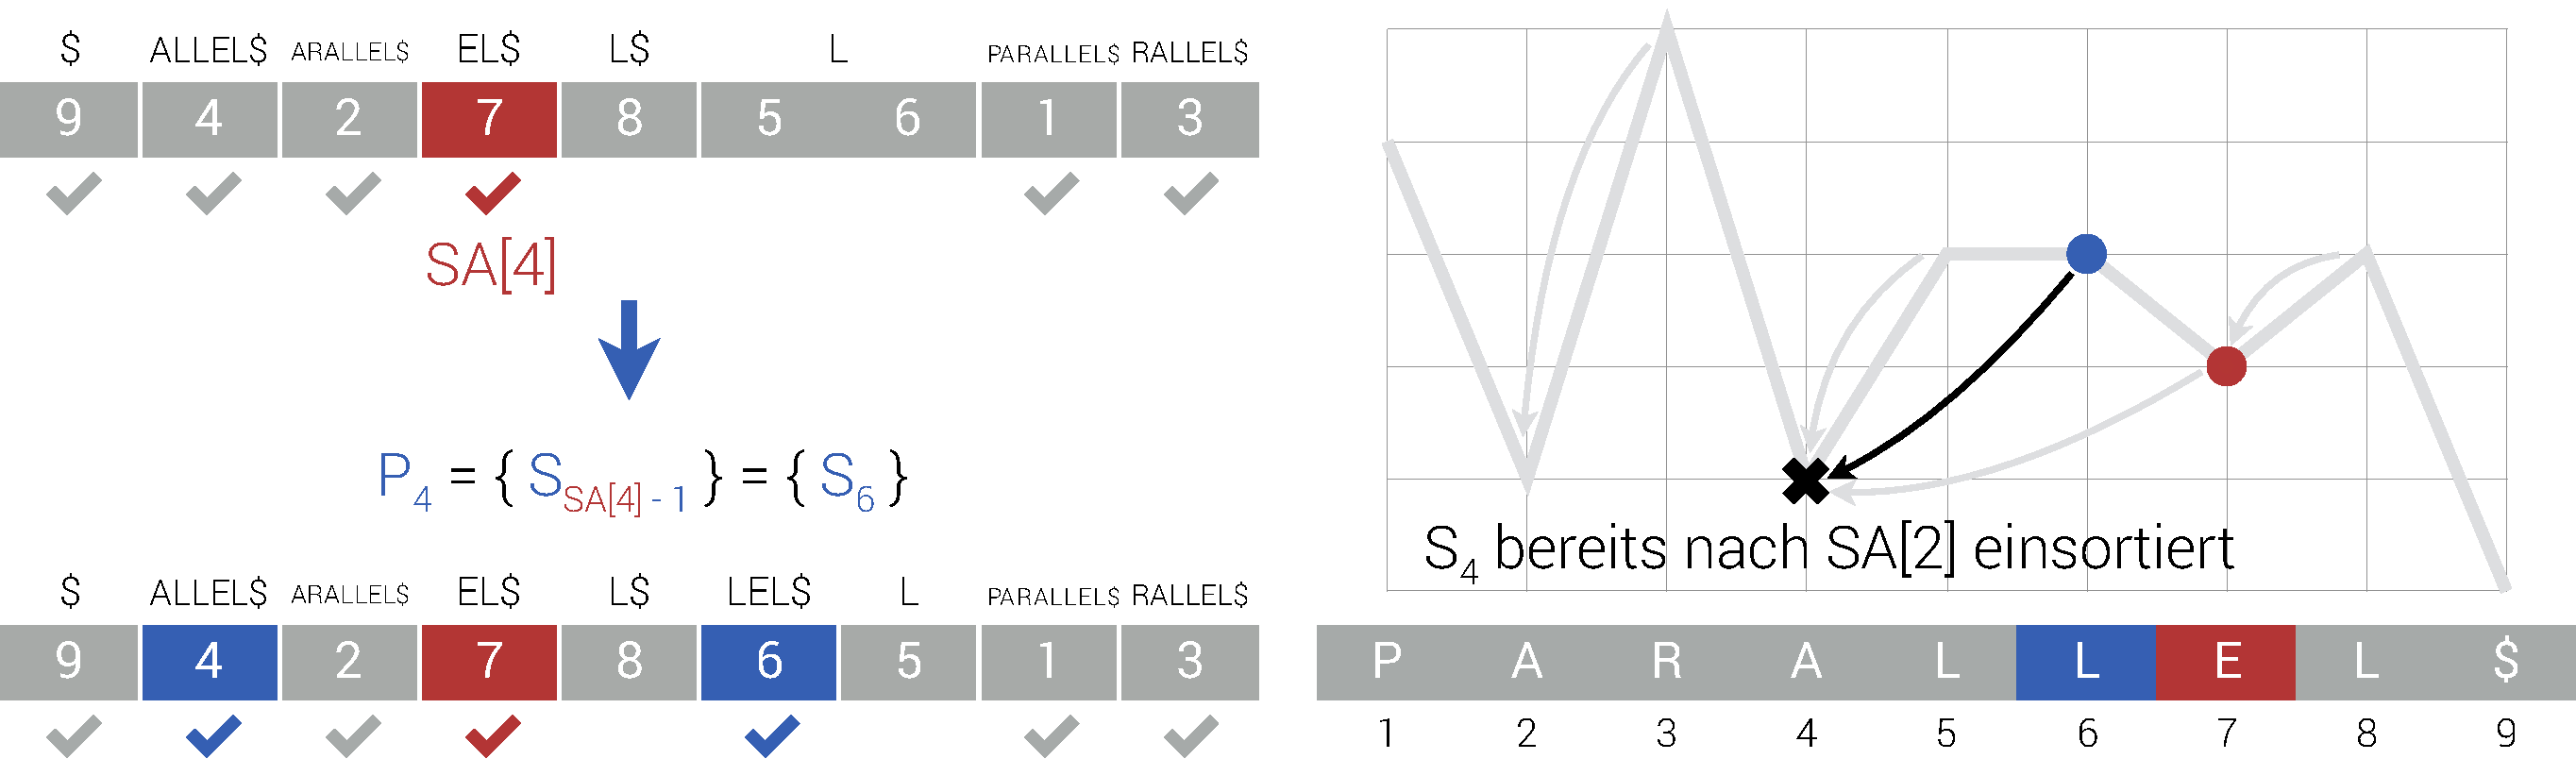
\includegraphics[width=\linewidth,bb=0 0 1310 386]{./assets/phase2-4.pdf}
	\caption{Iteration 4 von Phase 2: Berechnung und Einsortierung der $P_4$-Menge}
\label{fig:phase2-4}
\end{figure}

Es werden also alle alle Suffixe in $P_i$ aufgenommen, die auf der $prev$-Pointer-Kette liegen, die bei $S_{SA[i] - 1}$ beginnt, bis auf dieser Kette ein bereits einsortierter Suffix erreicht wird. Eine Intuition für die Korrektheit dieser Definition liefern diese zwei Überlegungen:

\begin{enumerate}
	\item Für $S_j \in P_i$ gilt, dass alle Suffixe zwischen $prev(j)$ und $j$ unmöglich in $P_i$ sein können, denn: $$\forall\ k \in \{ prev(j) + 1, \dots, j - 1 \}: S_j <_{lex} S_k \implies \widehat{k} \le j < \widehat{j} = i \implies S_k \notin P_i$$
	\item Falls beim Iterieren über die $prev$-Pointer-Kette ein Suffix $S_j$ erreicht wird, der bereits in $SA$ einsortiert wurde, kann dieser und alle noch in der Kette folgenden Suffixe unmöglich in $P_i$ liegen. Offensichtlich gilt, dass $S_j \notin P_i$, da auf den Kontext von $S_j$ ein anderer Suffix $S_l <_{lex} S_{SA[i]}$ folgen muss, sonst wäre $S_j$ nicht bereits einsortiert worden. Durch einen Widerspruchsbeweis lässt sich zeigen, dass alle Suffixe vor $S_j$ ebenfalls nicht in $P_i$ enthalten sein können. Der Beweis wird hier ausgelassen.
\end{enumerate}

Da jedem Suffix höchstens einmal entlang einer $prev$-Pointer-Kette gefolgt wird – danach wird er schließlich in $SA$ einsortiert und beendet ab dann weitere $prev$-Pointer-Ketten – und es $n$ Suffixe gibt, werden in Phase 2 für das Berechnen der $P_i$-Mengen also insgesamt $\mathcal{O}(n)$ Schritte benötigt. Beide Phasen laufen somit in Linearzeit, was GSACA zu einem rekursionsfreien Linearzeit-Suffix-Sorting-Algorithmus macht.

\begin{figure}[h]
	\centering
	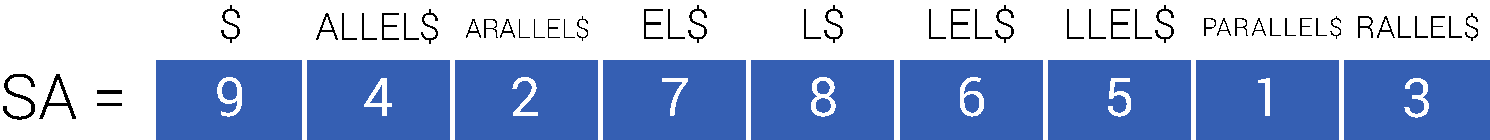
\includegraphics[width=0.6\linewidth,bb=0 0 715 67]{./assets/phase2Result.pdf}
	\caption{Ergebnis von Phase 2: Das Suffixarray $SA$ für $S =$ `parallel'}
\label{fig:phase2Result}
\end{figure}

\section{Performanceanalyse}

Nachdem nun erklärt wurde, die GSACA funktioniert, wird im Folgenden die Performance mit anderen SACAs verglichen.

\paragraph{Speicherbedarf} In der GSACA-Referenzimplementation~\cite{gsacaImplementation}, die im Rahmen der ursprünglichen Masterarbeit entstanden ist, wird, zusätzlich zum Speicher für Eingabe und Ausgabearray, $12n$ Speicher benötigt. Die rekursionsfreie Natur von GSACA bringt im Vergleich zu z.~B. SAIS aktuell also keinen Speichervorteil.

\begin{table}[h]
\begin{center}
\begin{tabular}{r | c c c}
& Skew & SAIS & \textbf{GSACA} \\
\hline
Art & \textcolor{rot}{rekursiv} & \textcolor{rot}{rekursiv} & \textcolor{gruen}{iterativ} \\
Zeit & $\mathcal{O}(n)$ & $\mathcal{O}(n)$ & $\mathcal{O}(n)$ \\
Speicher & $\textcolor{rot}{\mathcal{O}(\log n)} + \max 24n$ & $\textcolor{rot}{\mathcal{O}(\log n)} + \max 2n$ & $\textcolor{gruen}{\mathcal{O}(1)} + \textcolor{rot}{12n}$
\end{tabular}

\caption{Vergleich von Skew, SAIS und GSACA}
\label{tab:skewSaisGsacaComparison2}
\end{center}
\end{table}
\paragraph{Geschwindigkeit} Wie Abbildung~\ref{fig:performance} zeigt, kann GSACA aktuell auch im Hinblick auf seine Sortiergeschwindigkeit noch nicht mit dem state of the art SAIS Verfahren mithalten. Dies liegt zum einen daran, dass die Implementationen von SAIS im Laufe der letzten Jahre stärker optimiert werden konnten. Da GSACA noch ein sehr junges Verfahren ist, wurde noch nicht genug Zeit in das Finden einer bestmöglichen Implementation investiert. Ein weiterer Grund für das schlechte Abschneiden von GSACA ist, dass durch das viele nicht-lokale Springen zwischen Suffixen, z.~B. beim Pointer-Jumping, viele Cache-Misses produziert werden.

\begin{figure}[h]
	\centering
	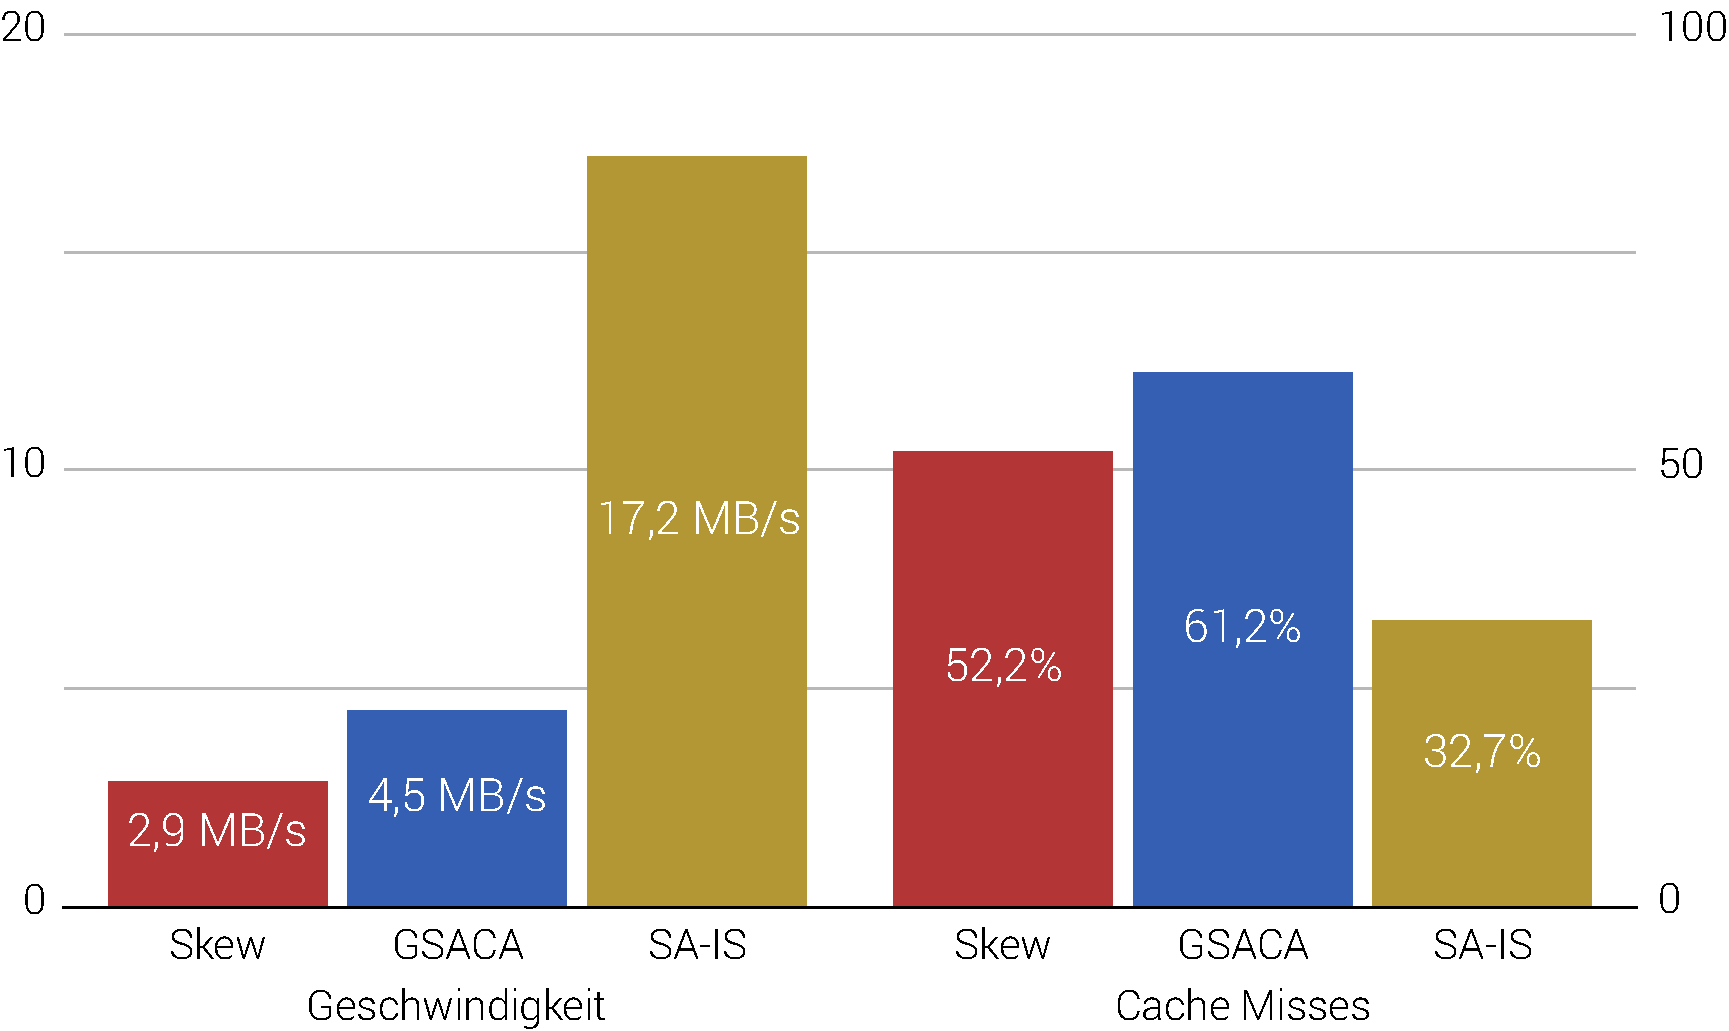
\includegraphics[width=0.6\linewidth,bb=0 0 830 495]{./assets/performance.pdf}
	\caption{Geschwindingkeit von GSACA im Vergleich, Testdaten: Silesia Corpus}
\label{fig:performance}
\end{figure}

Die Testergebnisse stammen aus der ursprünglichen GSACA-Masterarbeit und wurden unter Ubuntu 14.04.3 LTS (Kernel 3.13) auf einem Intel Xeon E5-2680v2 mit 2,8 GHz und 128 GB Hauptspeicher durchgeführt.

\section{Fazit}

Wie soeben in der Performanceanalyse gezeigt, ist GSACA aktuell noch nicht praxistauglich. Dies liegt allerdings vielmehr an der Neuheit des Verfahrens, als an der fundamentalen Untauglichkeit der verwendeten Ideen. Im Rahmen zukünftiger Forschung könnte beispielsweise versucht werden durch eine Stack-basierte Organisation der Daten das erwähnte Cache-Miss-Problem zu lösen, da wegen der $prev$-Pointer und der $\widehat{i}$ basierten Kontexte viel mit vorher/nachher-Relationen gearbeitet wird. Detaillierte Verbesserungsideen existieren allerdings noch nicht. GSACA ist aktuell also als Ausgangspunkt für weitere Forschung zu sehen.

\addcontentsline{toc}{section}{Literaturverzeichnis}
\bibliographystyle{plainnat}
\bibliography{paper}

\end{document}
